
\section{\textit{Contract Net}}\label{appendix:contract_net}
\subsection{Contexto}

O exemplo a seguir baseia-se na venda e compra de livros entre agentes vendedores (instâncias da classe \textit{BookSellerAgent}) e agentes compradores (instâncias da classe \textit{BookBuyerAgent}). 

Sob a perspectiva do agente comprador, este recebe o título do livro a ser comprado como um argumento em linha de comando e solicita periodicamente a todos os agentes vendedores que ofereçam uma oferta. Assim que uma oferta é recebida, o agente comprador aceita e emite uma ordem de compra. 

Se mais de um agente vendedor oferecer uma oferta, o comprador compara os preços e realiza a compra do livro mais barato. Tendo comprado o livro, o agente do comprador termina. 

Sob a perspectiva do agente vendedor, este possui uma interface, através da classe \textit{BookSellerGui}, na qual o usuário pode inserir novos títulos e seus respectivos preços. Ao receber solicitações para fornecer uma proposta para um livro, eles verificam se possui o título solicitado, podendo responder com o preço caso o possua, ou recusando-se a fazer uma proposta caso não o possua. Em caso de enviar uma proposta com o preço e de receber uma ordem de compra, o livro é vendido e removido do catálogo.

\subsection{Preparação do ambiente}

O exemplo foi rodado em sistema operacional Ubuntu 16.04, utilizando a IDE Eclipse Neon versão 4.6.3. Os seguintes passos devem ser seguidos para rodar este exemplo:

\begin{enumerate}
    \item Realizar o \textit{download} do arquivo \textit{jadeAll.zip} em \textit{http://jade.tilab.com/download/jade/}\footnote{Último acesso: Junho 2017} e descompactá-lo, bem como descompactar as pastas que encontram-se dentro do mesmo;
    \item Editar o arquivo \textit{.bashrc}. Para isso, executar o comando \textit{nano .bashrc} e adicionar as linhas abaixo ao final do arquivo. Substituir \textit{/caminho/para-o/jade} com a localização da pasta jade no computador. Por fim, salvar a edição. 
\begin{lstlisting}[numbers=none, language=bash]
#jade
export JADE_LIB=/caminho/para-o/jade
export JADE_CP=$JADE_LIB/http.
jar:$JADE_LIB/iiop.
jar:$JADE_LIB/jade.
jar:$JADE_LIB/jadeTools.
jar:
$JADE_LIB/commons-codec/commons-codec-1.3.
jar
alias rJade='
java -cp $JADE_CP jade.Boot'
alias cJade='
javac -cp $JADE_CP'
\end{lstlisting}
    \item Importar o código \textit{bookTrading}, presente na pasta \textit{jade/jade-examples/src/examples/bookTrading}, para o Eclipse.
    \item Selecionar \textit{Java Build Path > Libraries > Add External JARs}.
    \item Adicionar as seguintes bibliotecas do JADE ao projeto:
    \begin{itemize}
        \item \textit{jade/jade-src/lib/commons-codec/commons-codec-
1.3.jar};
        \item \textit{jade/jade-bin/lib/jade.jar}; 
        \item \texit{jade/jade-examples/lib/jadeExamples.jar}.
    \end{itemize}
    \item Selecionar \textit{Run > Run Configurations > Java Application}.
    \item Certificar que os seguintes parâmetros estão correspondentes aos valores a seguir:
    \begin{itemize}
        \item \textit{Project: BookAgents}
        \item \textit{Main class: jade.Boot}
    \end{itemize}
    \item Na aba \textit{Arguments} inserir, em \textit{Program Arguments}, o seguinte texto:
    \textit{-nomtp -gui bookSeller1:sell.BookSellerAgent; bookSeller2:sell.BookSellerAgent; bookBuyer1:sell.BookBuyerAgent("O colecionador");}
    \item Selecionar \textit{Aplly > Run}.
\end{enumerate}


\subsection{Classe \textit{BookSellerAgent}}

Para criar um agente JADE, define-se, basicamente, uma subclasse da classe \textit{jade.core.Agent}\footnote{http://jade.tilab.com/doc/api/jade/core/Agent.html (último acesso: Junho 2017)} que implementa-se o método \textit{setup()} e os comportamentos do agente. Por meio da  classe {jade.core.Agent}, os agentes podem realizar operações básicas da plataforma como registro, configuração, e troca de mensagens. Através do método \textit{setup()}, um agente registra seus serviços nas páginas amarelas e adiciona seus comportamentos.

Inicialmente, cria-se um catálogo de livros e a interface gráfica para o registro dos mesmos através da classe \textit{BookSellerGui}.

\begin{lstlisting}[firstnumber=37]
public class BookSellerAgent extends Agent {
	// The catalogue of books for sale (maps the title of a book to its price)
	private Hashtable catalogue;
	// The GUI by means of which the user can add books in the catalogue
	private BookSellerGui myGui;

	// Put agent initializations here
	protected void setup() {
		// Create the catalogue
		catalogue = new Hashtable();

		// Create and show the GUI 
		myGui = new BookSellerGui(this);
		myGui.showGui();
\end{lstlisting}

Em seguida, registra-se o serviço de venda de livros (um serviço do tipo \textit{Book-selling}) nas páginas amarelas para que esteja disponível para outros agentes. Para publicar seus serviços, um agente deve inscrever-se no agente DF (\textit{Directory Facilitator agent}). O DF reune e associa descrições de serviço aos seus identificadores (AID, \textit{Agent Identifier}); de modo que os agentes visitantes possam contactá-lo à procura de agentes que prestam os serviços de que necessitam. 

O padrão FIPA estabelece que cada instância de agente é identificada pelo AID (\textit{Agent Identifier}). Na plataforma JADE, um AID é uma instância da classe \textit{jade.core.AID}. Esta provê o método \textit{getAID()} que retorna o nome global do agente na plataforma no seguinte formato: \textit{<nome\_local>@<nome-plataforma>}.

O agente deve, portanto, fornecer seu AID e uma lista de seus serviços fornecidos através de uma descrição adequada, como uma instância da classe DFAgentDescription\footnote{http://jade.tilab.com/doc/api/jade/domain/FIPAAgentManagement/DFAgentDescription.html (último acesso: Junho 2017)} e, ao final, invocar o método estático \textit{register()} da classe DFService\footnote{http://jade.tilab.com/doc/api/jade/domain/DFService.html (último acesso: Junho 2017)}. 

\begin{lstlisting}[firstnumber=52]
		// Register the book-selling service in the yellow pages
		DFAgentDescription dfd = new DFAgentDescription();
		dfd.setName(getAID());
		ServiceDescription sd = new ServiceDescription();
		sd.setType("book-selling");
		sd.setName("JADE-book-trading");
		dfd.addServices(sd);
		try {
			DFService.register(this, dfd);
		}
		catch (FIPAException fe) {
			fe.printStackTrace();
		}
\end{lstlisting}

Por fim, ainda no método \textit{setup()}, são adicionados os comportamentos que atendem às consultas dos agentes compradores (através da classe \textit{OfferRequestsServer} e os comportamentos que atendem às ordens de compra dos agentes compradores (através da classe \textit{PurchaseOrdersServer}).

\begin{lstlisting}[firstnumber=66]
		// Add the behaviour serving queries from buyer agents
		addBehaviour(new OfferRequestsServer());

		// Add the behaviour serving purchase orders from buyer agents
		addBehaviour(new PurchaseOrdersServer());
	}
\end{lstlisting}

Além do método \textit{setup()}, a classe possui o método \textit{takeDown()} que é invocado imediatamente antes de um agente ter encerrado seus serviços com objetivo de executar várias operações de limpeza.

\begin{lstlisting}[firstnumber=73]
	// Put agent clean-up operations here
	protected void takeDown() {
		// Deregister from the yellow pages
		try {
			DFService.deregister(this);
		}
		catch (FIPAException fe) {
			fe.printStackTrace();
		}
		// Close the GUI
		myGui.dispose();
		// Printout a dismissal message
		System.out.println("Seller-agent "+getAID().getName()+" terminating.");
	}
\end{lstlisting}

A classe \textit{OfferRequestsServer} implementa um dos comportamentos da classe \textit{BookSellerAgent}. Ao extender a classe \textit{jade.core.behaviours.CyclicBehaviour}\footnote{http://jade.tilab.com/doc/api/jade/core/behaviours/CyclicBehaviour.html (último acesso: Junho 2017)}, o método \textit{action()} repete-se à medida que o \textit{setup()} invoque-o. Através deste comportamento, o agente vendedor pode atender aos pedidos de oferta recebidos de agentes compradores.

Uma instância da classe \textit{jade.lang.acl.MessageTemplate}\footnote{http://jade.tilab.com/doc/api/jade/lang/acl/MessageTemplate.html (último acesso: Junho 2017)} possibilita que as mensagens recebidas pelo agente vendedor sejam filtradas. Esta classe especifica templates para serem usados ao chamar o método \textit{receive()}. Quando um modelo é especificado, o método \textit{receive()} retorna a primeira correspondência da mensagem, se houver, e ignora todas as mensagens não correspondentes. 

Cabe ressaltar que toda mensagem corresponde a instâncias da classe ACLMessage\footnote{http://jade.cselt.it/doc/api/jade/lang/acl/ACLMessage.html (último acesso: Junho 2017)}. Esta classe implementa o padrão FIPA-ACL e, assim, disponibiliza um conjunto de atributos que estão de acordo com as especificações FIPA.

Neste caso, espera-se receber a performativa CFP (\textit{Call For Proposal}) onde o agentes compradores solicitam propostas aos agentes vendedores especificando o nome do livro que desejam comprar. Se o livro solicitado estiver disponível no catálogo local, o agente vendedor responde com uma mensagem \textit{PROPOSE} especificando o preço. Caso contrário, uma mensagem \textit{REFUSE} é enviada. 

\begin{lstlisting}[firstnumber=108]
	private class OfferRequestsServer extends CyclicBehaviour {
		public void action() {
			MessageTemplate mt = MessageTemplate.MatchPerformative(ACLMessage.CFP);
			ACLMessage msg = myAgent.receive(mt);
			if (msg != null) {
				// CFP Message received. Process it
				String title = msg.getContent();
				ACLMessage reply = msg.createReply();

				Integer price = (Integer) catalogue.get(title);
				if (price != null) {
					// The requested book is available for sale. Reply with the price
					reply.setPerformative(ACLMessage.PROPOSE);
					reply.setContent(String.valueOf(price.intValue()));
				}
				else {
					// The requested book is NOT available for sale.
					reply.setPerformative(ACLMessage.REFUSE);
					reply.setContent("not-available");
				}
				myAgent.send(reply);
			}
			else {
				block();
			}
		}
	}  // End of inner class OfferRequestsServer
\end{lstlisting}


De modo semelhante, a classe \textit{PurchaseOrdersServer} também especifica um comportamento do tipo \textit{CyclicBehaviour} e aguarda o recebimento de uma performativa específica: \textit{ACCEPT\_PROPOSAL}. Esta é recebida quando o agente comprador aceita a proposta e a venda do livro pode, portanto, ser processada. O agente vendedor remove o livro comprado de seu catálogo e responde com uma mensagem \textit{INFORM} para notificar o comprador de que a compra foi concluída.


\begin{lstlisting}[firstnumber=144]
	private class PurchaseOrdersServer extends CyclicBehaviour {
		public void action() {
			MessageTemplate mt = MessageTemplate.MatchPerformative(ACLMessage.ACCEPT_PROPOSAL);
			ACLMessage msg = myAgent.receive(mt);
			if (msg != null) {
				// ACCEPT_PROPOSAL Message received. Process it
				String title = msg.getContent();
				ACLMessage reply = msg.createReply();

				Integer price = (Integer) catalogue.remove(title);
				if (price != null) {
					reply.setPerformative(ACLMessage.INFORM);
					System.out.println(title+" sold to agent "+msg.getSender().getName());
				}
				else {
					// The requested book has been sold to another buyer in the meanwhile .
					reply.setPerformative(ACLMessage.FAILURE);
					reply.setContent("not-available");
				}
				myAgent.send(reply);
			}
			else {
				block();
			}
		}
	}  // End of inner class OfferRequestsServer
}
\end{lstlisting}


		

\subsection{Classe \textit{BookBuyerAgent}}

A classe \textit{BookBuyerAgent} implementa os comportamentos relacionados à compra do livro de interesse do agente comprador. No método \textit{setup()}, adiciona-se um comportamento do tipo \textit{TickerBehaviour}\footnote{http://jade.tilab.com/doc/api/jade/core/behaviours/TickerBehaviour.html (último acesso: Junho 2017)}. Esta classe possibilita que execute-se um trecho de código por um período de tempo pré-definido por meio do método \textit{onTick()}. Para este caso, foi definida a duração de um minuto.

Uma instância da classe \textit{ServiceDescription}\footnote{http://jade.tilab.com/doc/api/jade/domain/FIPAAgentManagement/ServiceDescription.html (último acesso: Junho 2017)} é criada para definir um serviço do tipo  \textit{book-selling}, para que, através de uma instância da classe \textit{DFAgentDescription()}, sejam buscados agentes vendedores que possuam em seu catálogo o \textit{targetBookTitle}. Por fim, os AIDs dos agentes que prestam o serviço solicitado são salvos em uma lista chamada \textit{sellerAgents}.

\begin{lstlisting}[firstnumber=36]
public class BookBuyerAgent extends Agent {
	// The title of the book to buy
	private String targetBookTitle;
	// The list of known seller agents
	private AID[] sellerAgents;

	// Put agent initializations here
	protected void setup() {
		// Printout a welcome message
		System.out.println("Hallo! Buyer-agent "+getAID().getName()+" is ready.");

		// Get the title of the book to buy as a start-up argument
		Object[] args = getArguments();
		if (args != null && args.length > 0) {
			targetBookTitle = (String) args[0];
			System.out.println("Target book is "+targetBookTitle);

			// Add a TickerBehaviour that schedules a request to seller agents every minute
			addBehaviour(new TickerBehaviour(this, 60000) {
				protected void onTick() {
					System.out.println("Trying to buy "+targetBookTitle);
					// Update the list of seller agents
					DFAgentDescription template = new DFAgentDescription();
					ServiceDescription sd = new ServiceDescription();
					sd.setType("book-selling");
					template.addServices(sd);
					try {
						DFAgentDescription[] result = DFService.search(myAgent, template); 
						System.out.println("Found the following seller agents:");
						sellerAgents = new AID[result.length];
						for (int i = 0; i < result.length; ++i) {
							sellerAgents[i] = result[i].getName();
							System.out.println(sellerAgents[i].getName());
						}
					}
					catch (FIPAException fe) {
						fe.printStackTrace();
					}
\end{lstlisting}

Em seguida, o comportamento \textit{RequestPerformer} é adicionado ao agente comprador. 

\begin{lstlisting}[firstnumber=75]
					// Perform the request
					myAgent.addBehaviour(new RequestPerformer());
\end{lstlisting}

Caso nenhum livro tenha sido especificado, o agente é finalizado.

\begin{lstlisting}[firstnumber=80]
		else {
			// Make the agent terminate
			System.out.println("No target book title specified");
			doDelete();
		}
	}
\end{lstlisting}

Logo após, é definida a classe \textit{RequestPerformer}. Primeiramente, é enviada uma mensagem CFP para todos os agentes vendedores da lista \textit{sellerAgents}.  

\begin{lstlisting}[firstnumber=98]
	private class RequestPerformer extends Behaviour {
		private AID bestSeller; // The agent who provides the best offer 
		private int bestPrice;  // The best offered price
		private int repliesCnt = 0; // The counter of replies from seller agents
		private MessageTemplate mt; // The template to receive replies
		private int step = 0;

		public void action() {
			switch (step) {
			case 0:
				// Send the cfp to all sellers
				ACLMessage cfp = new ACLMessage(ACLMessage.CFP);
				for (int i = 0; i < sellerAgents.length; ++i) {
					cfp.addReceiver(sellerAgents[i]);
				} 
				cfp.setContent(targetBookTitle);
				cfp.setConversationId("book-trade");
				cfp.setReplyWith("cfp"+System.currentTimeMillis()); // Unique value
				myAgent.send(cfp);
				// Prepare the template to get proposals
				mt = MessageTemplate.and(MessageTemplate.MatchConversationId("book-trade"),
						MessageTemplate.MatchInReplyTo(cfp.getReplyWith()));
				step = 1;
				break;
\end{lstlisting}

Em seguida, todas as mensagens recebidas são lidas. Aquelas cujas performativas correspondem a \textit{PROPOSE}, têm seu conteúdo lido, o que corresponde ao preço do livro. Logo após, os preços são comparados até que se encontre o mais barato (\textit{bestPrice}). 

\begin{lstlisting}[firstnumber=122]
			case 1:
				// Receive all proposals/refusals from seller agents
				ACLMessage reply = myAgent.receive(mt);
				if (reply != null) {
					// Reply received
					if (reply.getPerformative() == ACLMessage.PROPOSE) {
						// This is an offer 
						int price = Integer.parseInt(reply.getContent());
						if (bestSeller == null || price < bestPrice) {
							// This is the best offer at present
							bestPrice = price;
							bestSeller = reply.getSender();
						}
					}
					repliesCnt++;
					if (repliesCnt >= sellerAgents.length) {
						// We received all replies
						step = 2; 
					}
				}
				else {
					block();
				}
				break;
\end{lstlisting}

Em seguida, é enviado o pedido ao vendedor que forneceu a melhor oferta (\textit{bestSeller}) através da performativa \textit{ACCEPT\_PROPOSAL}.

\begin{lstlisting}[firstnumber=146]
			case 2:
				// Send the purchase order to the seller that provided the best offer
				ACLMessage order = new ACLMessage(ACLMessage.ACCEPT_PROPOSAL);
				order.addReceiver(bestSeller);
				order.setContent(targetBookTitle);
				order.setConversationId("book-trade");
				order.setReplyWith("order"+System.currentTimeMillis());
				myAgent.send(order);
				// Prepare the template to get the purchase order reply
				mt = MessageTemplate.and(MessageTemplate.MatchConversationId("book-trade"),
						MessageTemplate.MatchInReplyTo(order.getReplyWith()));
				step = 3;
				break;
\end{lstlisting}

A performativa \textit{INFORM} significa, neste caso, que a compra foi executada com êxito. Caso receba qualquer outra mensagem, significa que a tentativa de compra falhou.

\begin{lstlisting}[firstnumber=159]
			case 3:      
				// Receive the purchase order reply
				reply = myAgent.receive(mt);
				if (reply != null) {
					// Purchase order reply received
					if (reply.getPerformative() == ACLMessage.INFORM) {
						// Purchase successful. We can terminate
						System.out.println(targetBookTitle+" successfully purchased from agent "+reply.getSender().getName());
						System.out.println("Price = "+bestPrice);
						myAgent.doDelete();
					}
					else {
						System.out.println("Attempt failed: requested book already sold.");
					}

					step = 4;
				}
				else {
					block();
				}
				break;
			}        
		}
\end{lstlisting}


\subsection{Resultados da execução}


A Figura \ref{fig:book-trading00} apresenta a inicialização do contêiner e dos serviços da plataforma JADE. A Figura \ref{fig:book-trading01} apresenta a plataforma JADE e a estrutura do contêiner. 


\begin{figure}[h]
\centering
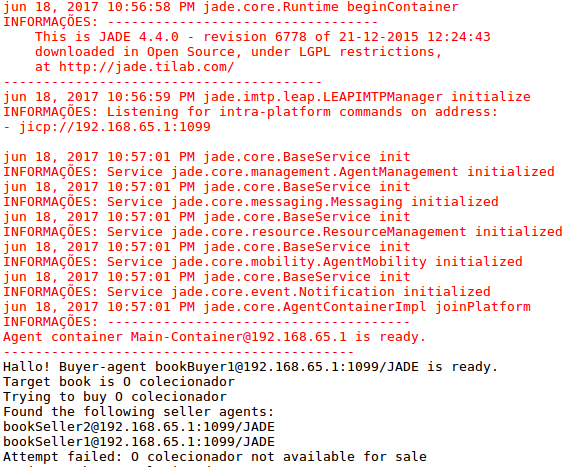
\includegraphics[scale=0.6]{figuras/contract-net/book-trading00}
\caption{Saídas do console: inicialização da plataforma.}
\label{fig:book-trading00}
\end{figure}

\begin{figure}[H]
\centering
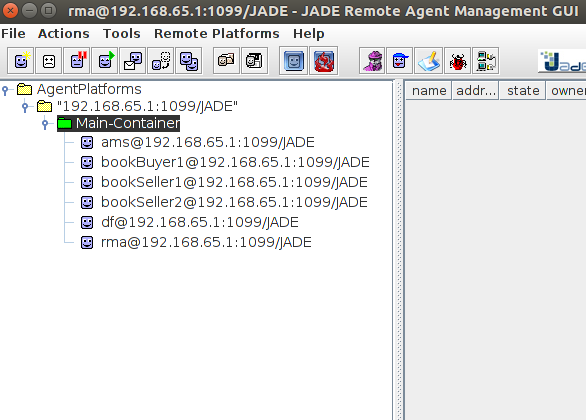
\includegraphics[scale=0.5]{figuras/contract-net/book-trading01}
\caption{Plataforma JADE}
\label{fig:book-trading01}
\end{figure}

A Figura \ref{fig:book-trading02} apresenta o comportamento cíclico do agente comprador, que realiza várias tentativas de compra do livro a cada minuto.

\begin{figure}[H]
\centering
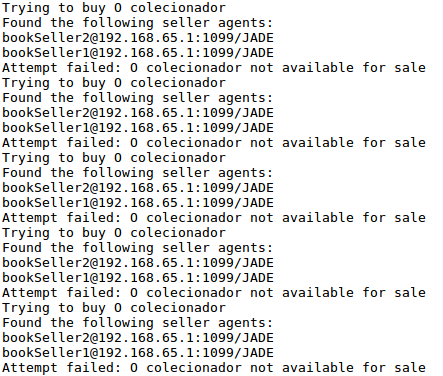
\includegraphics[scale=0.55]{figuras/contract-net/book-trading02}
\caption{Saídas do console: tentativas de compra do agente comprador}
\label{fig:book-trading02}
\end{figure}

Ao inserir no catálogo o livro procurado pelo agente comprador (Figura \ref{fig:book-trading03}), o agente comprador encontra o livro desejado e realiza sua compra (Figura \ref{fig:book-trading04}).

\begin{figure}[!h]
\centering
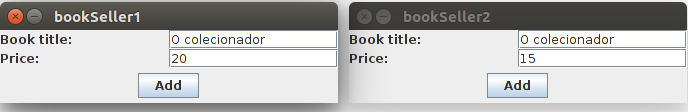
\includegraphics[scale=0.4]{figuras/contract-net/book-trading03}
\caption{Interface para catalogação dos livros.}
\label{fig:book-trading03}
\end{figure}

\begin{figure}[!h]
\centering
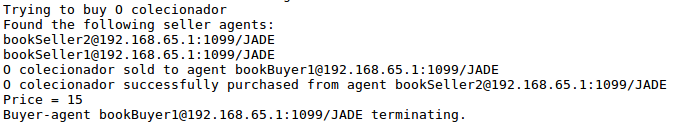
\includegraphics[scale=0.55]{figuras/contract-net/book-trading04}
\caption{Saídas do console: finalização da compra.}
\label{fig:book-trading04}
\end{figure}